\section{Results}
\label{sec:results}

\subsection{Headline: three-way diagnostic accuracy}
\label{sec:headline}

\Tabref{tab:main} reports the three-way diagnostic accuracy on the held-out test
set ($n = 3{,}000$). The hybrid reaches a \macrofone of $\mathbf{0.991}$
($[0.987, 0.994]$), decisively beating every single-modality baseline:
\symonly{} $0.871$, \bayonly{} $0.489$, \tostonly{} $0.326$, and \nhst{} $0.244$.
That is a $+0.12$ gain over the strongest single modality and more than a
$4\times$ improvement over the naive baseline. The hybrid's bootstrap confidence
interval does not overlap any baseline's, and \figref{fig:macroF1} shows the
intervals are cleanly separated.

\begin{table}[t]
\centering
\caption{Three-way cause-classification on the held-out test set ($n=3{,}000$,
classes $[1001,989,1010]$). Higher is better except ECE. \GR{}/\WI{}/\DF{} columns
are per-class F1. Best in \textbf{bold}. The hybrid dominates on every metric; the
two single modalities each collapse on a different class (\bayonly{} on \DF,
\symonly{} via robustness$\leftrightarrow$weak confusion reflected in its high
ECE). $^\dagger$The LLM judge is scored on a stratified 150-scenario subset; all
others on the full test set.}
\label{tab:main}
\resizebox{\textwidth}{!}{%
\begin{tabular}{@{}lccccccc@{}}
\toprule
\textbf{Method} & \textbf{\macrofone (95\% CI)} & \textbf{Acc} &
$\boldsymbol{\kappa}$ & \textbf{ECE} & \textbf{\GR{} F1} & \textbf{\WI{} F1} &
\textbf{\DF{} F1} \\
\midrule
\nhst{}        & 0.244 \,{\scriptsize [0.233, 0.257]} & 0.362 & ---   & ---   & --- & --- & 0.00 \\
\tostonly{}    & 0.326 \,{\scriptsize [0.312, 0.340]} & 0.424 & ---   & ---   & --- & --- & 0.00 \\
\bayonly{}     & 0.489 \,{\scriptsize [0.478, 0.499]} & 0.608 & 0.414 & 0.058 & 0.80 & 0.66 & 0.00 \\
\symonly{}     & 0.871 \,{\scriptsize [0.860, 0.883]} & 0.876 & 0.814 & 0.191 & 0.84 & 0.77 & \textbf{1.00} \\
\llmjudge{}$^\dagger$ & 0.888 & 0.887 & 0.830 & ---   & 0.85 & 0.85 & 0.97 \\
\midrule
\textbf{\hybrid{} (ours)} & \textbf{0.991} \,{\scriptsize [0.987, 0.994]} &
\textbf{0.991} & \textbf{0.986} & 0.248 & \textbf{0.99} & \textbf{0.99} &
\textbf{1.00} \\
\bottomrule
\end{tabular}
}
\end{table}

\begin{figure}[t]
\centering
\begin{subfigure}[b]{0.48\textwidth}
  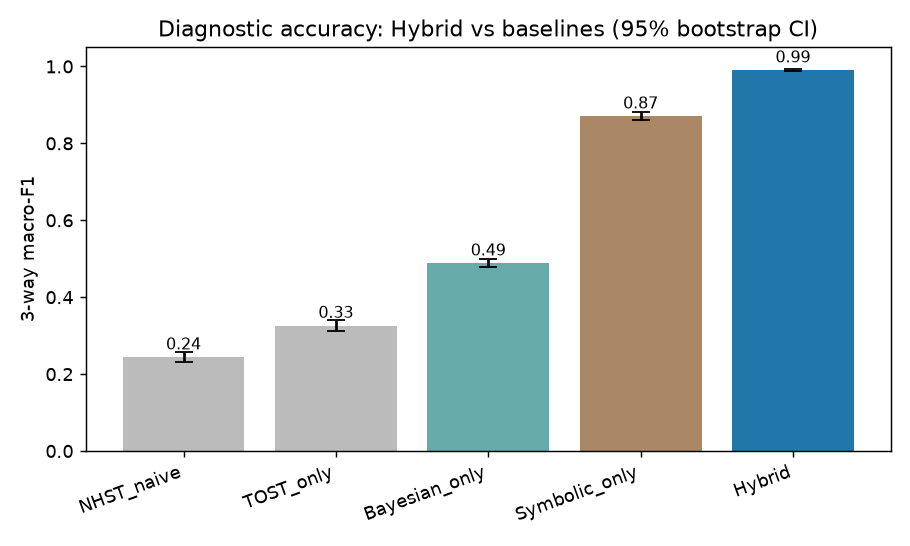
\includegraphics[width=\textwidth]{figures/fig1_macroF1.png}
  \caption{Macro-F1 with bootstrap CIs}
  \label{fig:macroF1}
\end{subfigure}
\hfill
\begin{subfigure}[b]{0.48\textwidth}
  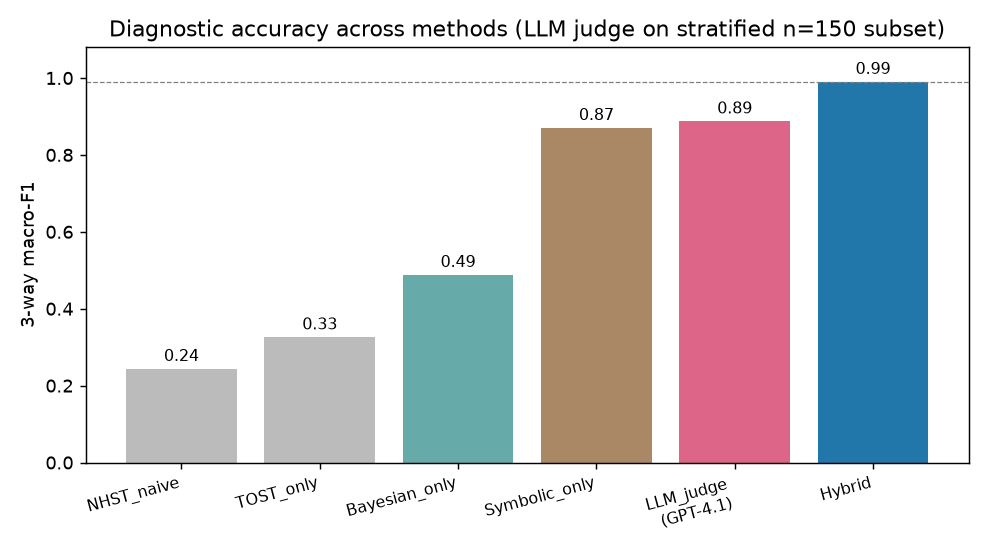
\includegraphics[width=\textwidth]{figures/fig4_all_methods.png}
  \caption{All methods incl.\ LLM judge}
  \label{fig:allmethods}
\end{subfigure}
\caption{\textbf{The hybrid dominates every baseline.} \captiona Three-way
\macrofone with $1{,}000$-resample bootstrap 95\% CIs; the hybrid's interval
$[0.987, 0.994]$ does not overlap any baseline's. \captionb Adding the frontier
LLM judge on the stratified subset leaves the ranking unchanged: the hybrid scores
$0.993$ there, above the LLM's $0.888$ and the symbolic baseline's $0.806$.}
\label{fig:headline}
\end{figure}

\para{Significance.} Under the McNemar exact test with Holm correction, the hybrid
beats \symonly{} at $p = 3.7\times10^{-78}$ (a net $+343$ correct cases), and beats
\bayonly{}, \tostonly{}, and \nhst{} all at $p < 10^{-300}$ (net $+1148$, $+1701$,
and $+1885$ cases respectively). Every comparison clears the corrected threshold
by a wide margin.

\subsection{Mechanism: where each modality is blind}
\label{sec:mechanism}

The confusion matrices in \figref{fig:confusion} explain \emph{why} the hybrid
wins, and confirm that the two modalities fail on disjoint, complementary slices.

\begin{figure}[t]
\centering
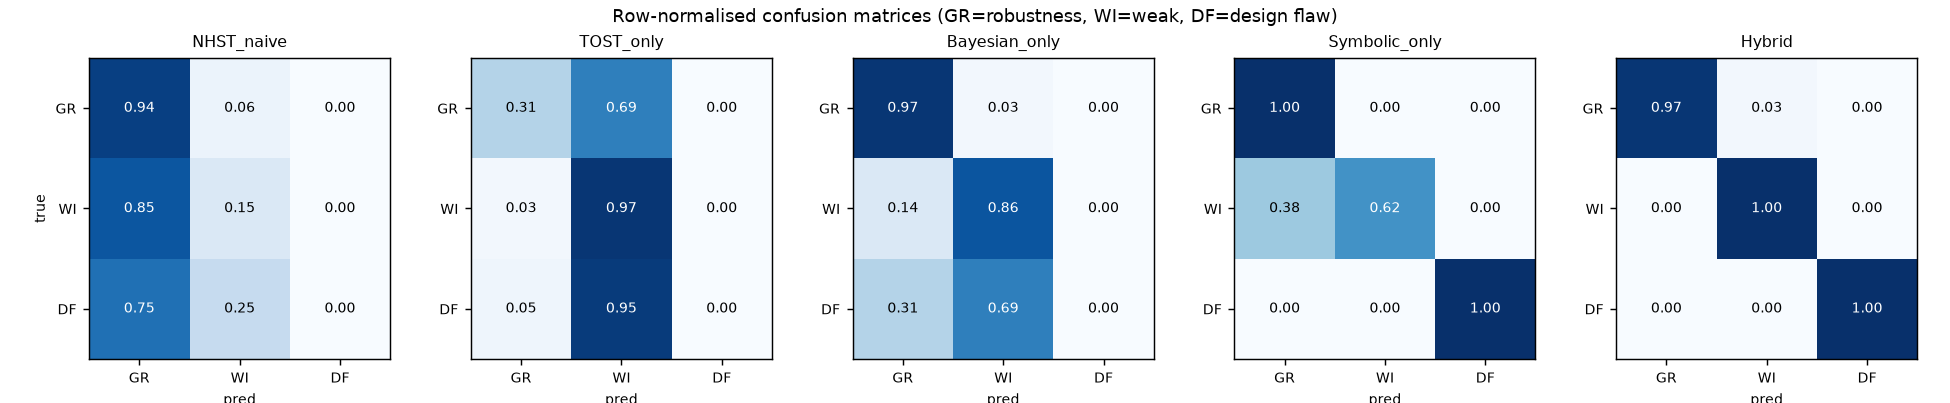
\includegraphics[width=0.95\linewidth]{figures/fig2_confusion.png}
\caption{\textbf{Row-normalised confusion matrices.} \bayonly{} (left) has no
concept of a structural flaw, so it routes all $1{,}010$ \DF{} nulls elsewhere
($310 \rightarrow$ \GR, $700 \rightarrow$ \WI) and never recovers one
($\textsc{F1}=0.00$). \symonly{} (center) gets design flaws perfectly but, blind to
$N$ and noise, mislabels $371/989$ underpowered cases as \GR. The hybrid (right)
resolves both, leaving only $28/3{,}000$ errors.}
\label{fig:confusion}
\end{figure}

\para{Bayesian-only is blind to design flaws.} Its \DF{} F1 is exactly $0.00$: all
$1{,}010$ design-flaw nulls are misrouted ($310 \rightarrow$ \GR,
$700 \rightarrow$ \WI). A confound that cancels a real effect, or a logically
unconfirmable point null, is simply invisible to evidence alone---confirming our
hypothesis that statistical evidence cannot see structural flaws.

\para{Symbolic-only is blind to power.} It gets design flaws perfectly
($\textsc{F1}=1.00$) but, unable to see $N$ or measurement noise, mislabels
$371/989$ underpowered (small-$N$ or coarse-metric) cases as \GR. This is the
robustness$\leftrightarrow$weak confusion we predicted, and is the reason its ECE
($0.191$) is high despite a respectable \macrofone.

\para{The hybrid resolves both.} Holding all the discriminating inputs---sample
size and noise from the Bayesian side, structural flags and intervention strength
from the symbolic side---the hybrid makes only $28/3{,}000$ errors: $27$ are
robustness$\leftrightarrow$weak boundary cases sitting near the noise/$N$
thresholds, and $1$ is the reverse. Design flaws are perfect. It is the only method
that observes every signal needed to separate all three causes.

\subsection{Interpretability}
\label{sec:interp}

Every diagnosis is a short reasoning chain that names the operative evidence and
the failed check. Three verbatim examples from the framework's output:
\begin{itemize}[leftmargin=*,itemsep=2pt,topsep=2pt]
  \item \textbf{\GR{}} (conf.\ $0.75$): ``[Symbolic gate] clean, identifiable \&
        confirmable design $\ldots$ [Bayesian] adequate sample ($n{=}100$) and
        precise measurement ($\mathrm{sd}{=}1.52$); [Symbolic] substantive
        intervention (strength$=0.64$) still found nothing
        ($\mathrm{BF}_{01}{=}5.50$) $\rightarrow$ \GR.''
  \item \textbf{\WI{}} (conf.\ $0.70$): ``$\ldots$ [Bayesian] inadequate sample
        ($n{=}20 < 50$) [Symbolic] weak intervention (strength$=0.17 < 0.5$)
        $\rightarrow$ a real effect could be masked $\rightarrow$ \WI.''
  \item \textbf{\DF{}} (conf.\ $0.84$): ``[Symbolic gate] Design-flaw gate fired:
        evaluation-awareness; non-identifiable. Structure uninterpretable
        $\rightarrow$ \DF.''
\end{itemize}
Because each diagnosis names the specific failed check, the output maps directly
to an action---increase $N$, strengthen the attack, or remove the confound /
specify an equivalence margin.

\subsection{External LLM judge}
\label{sec:llm}

A frontier general reasoner does not, on its own, match the structured framework.
Given identical information and an explicit rubric, \llmjudge{} scores
\macrofone $=0.888$ (Cohen's $\kappa = 0.83$ against ground truth)---competitive
with the symbolic baseline but clearly below the hybrid's $0.993$ on the
\emph{same} 150-scenario subset (\figref{fig:allmethods}; on that subset
\symonly{} scores $0.806$ and \bayonly{} $0.485$, so the ranking is unchanged). The
judge nails design flaws ($\textsc{F1}=0.97$, the flags are salient in text) but
still confuses robustness with weak intervention: it does not reliably convert
$N{=}20$ or $\mathrm{sd}{=}3.2$ into ``underpowered''. The framework's explicit
power and identifiability logic adds value the LLM does not supply for free, and
does so transparently and at near-zero marginal cost ($8.8$\,s versus $396$\,s of
API calls).

\subsection{Sensitivity and calibration}
\label{sec:sensitivity}

\figref{fig:sensitivity} sweeps the Bayes-factor Cauchy prior scale
$r \in \{0.354, 0.5, 0.707, 1.0, 1.414\}$. Hybrid \macrofone moves only within
$[0.989, 0.993]$, so the framework is robust to prior specification---the
detectable-effect branch is its only prior-dependent component. On calibration, the
hybrid's ECE of $0.248$ reflects \emph{under}-confidence (mean confidence
$\approx 0.74$ while accuracy is $0.99$). For a diagnostic tool this conservative
direction is the safer one; we revisit post-hoc calibration in
\secref{sec:discussion}.

\begin{figure}[t]
\centering
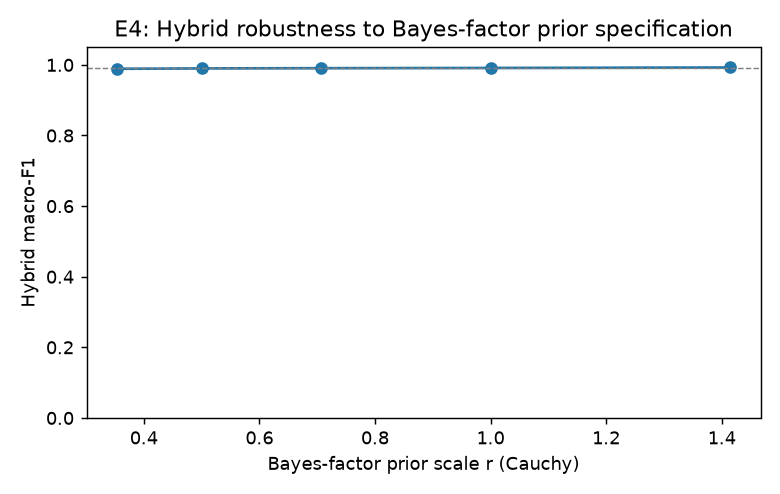
\includegraphics[width=0.6\linewidth]{figures/fig3_sensitivity.png}
\caption{\textbf{Robustness to the Bayes-factor prior.} Sweeping the Cauchy prior
scale $r$ moves hybrid \macrofone only within $[0.989, 0.993]$, confirming the
framework is insensitive to prior specification.}
\label{fig:sensitivity}
\end{figure}
